\section{Results \& Discussion}

\subsection{Orientation}
The frequency scan in \autoref{fig:frequency_scan} shows that apart from the large resonance peak at the crystal manufacturer's stated resonance frequency of $f_0 = \SI{4.606}{MHz}$, there are many smaller peaks corresponding to different resonance modes. The largest response is not necessarily the most useful response for this experiment. 

\begin{figure}
	\centering
		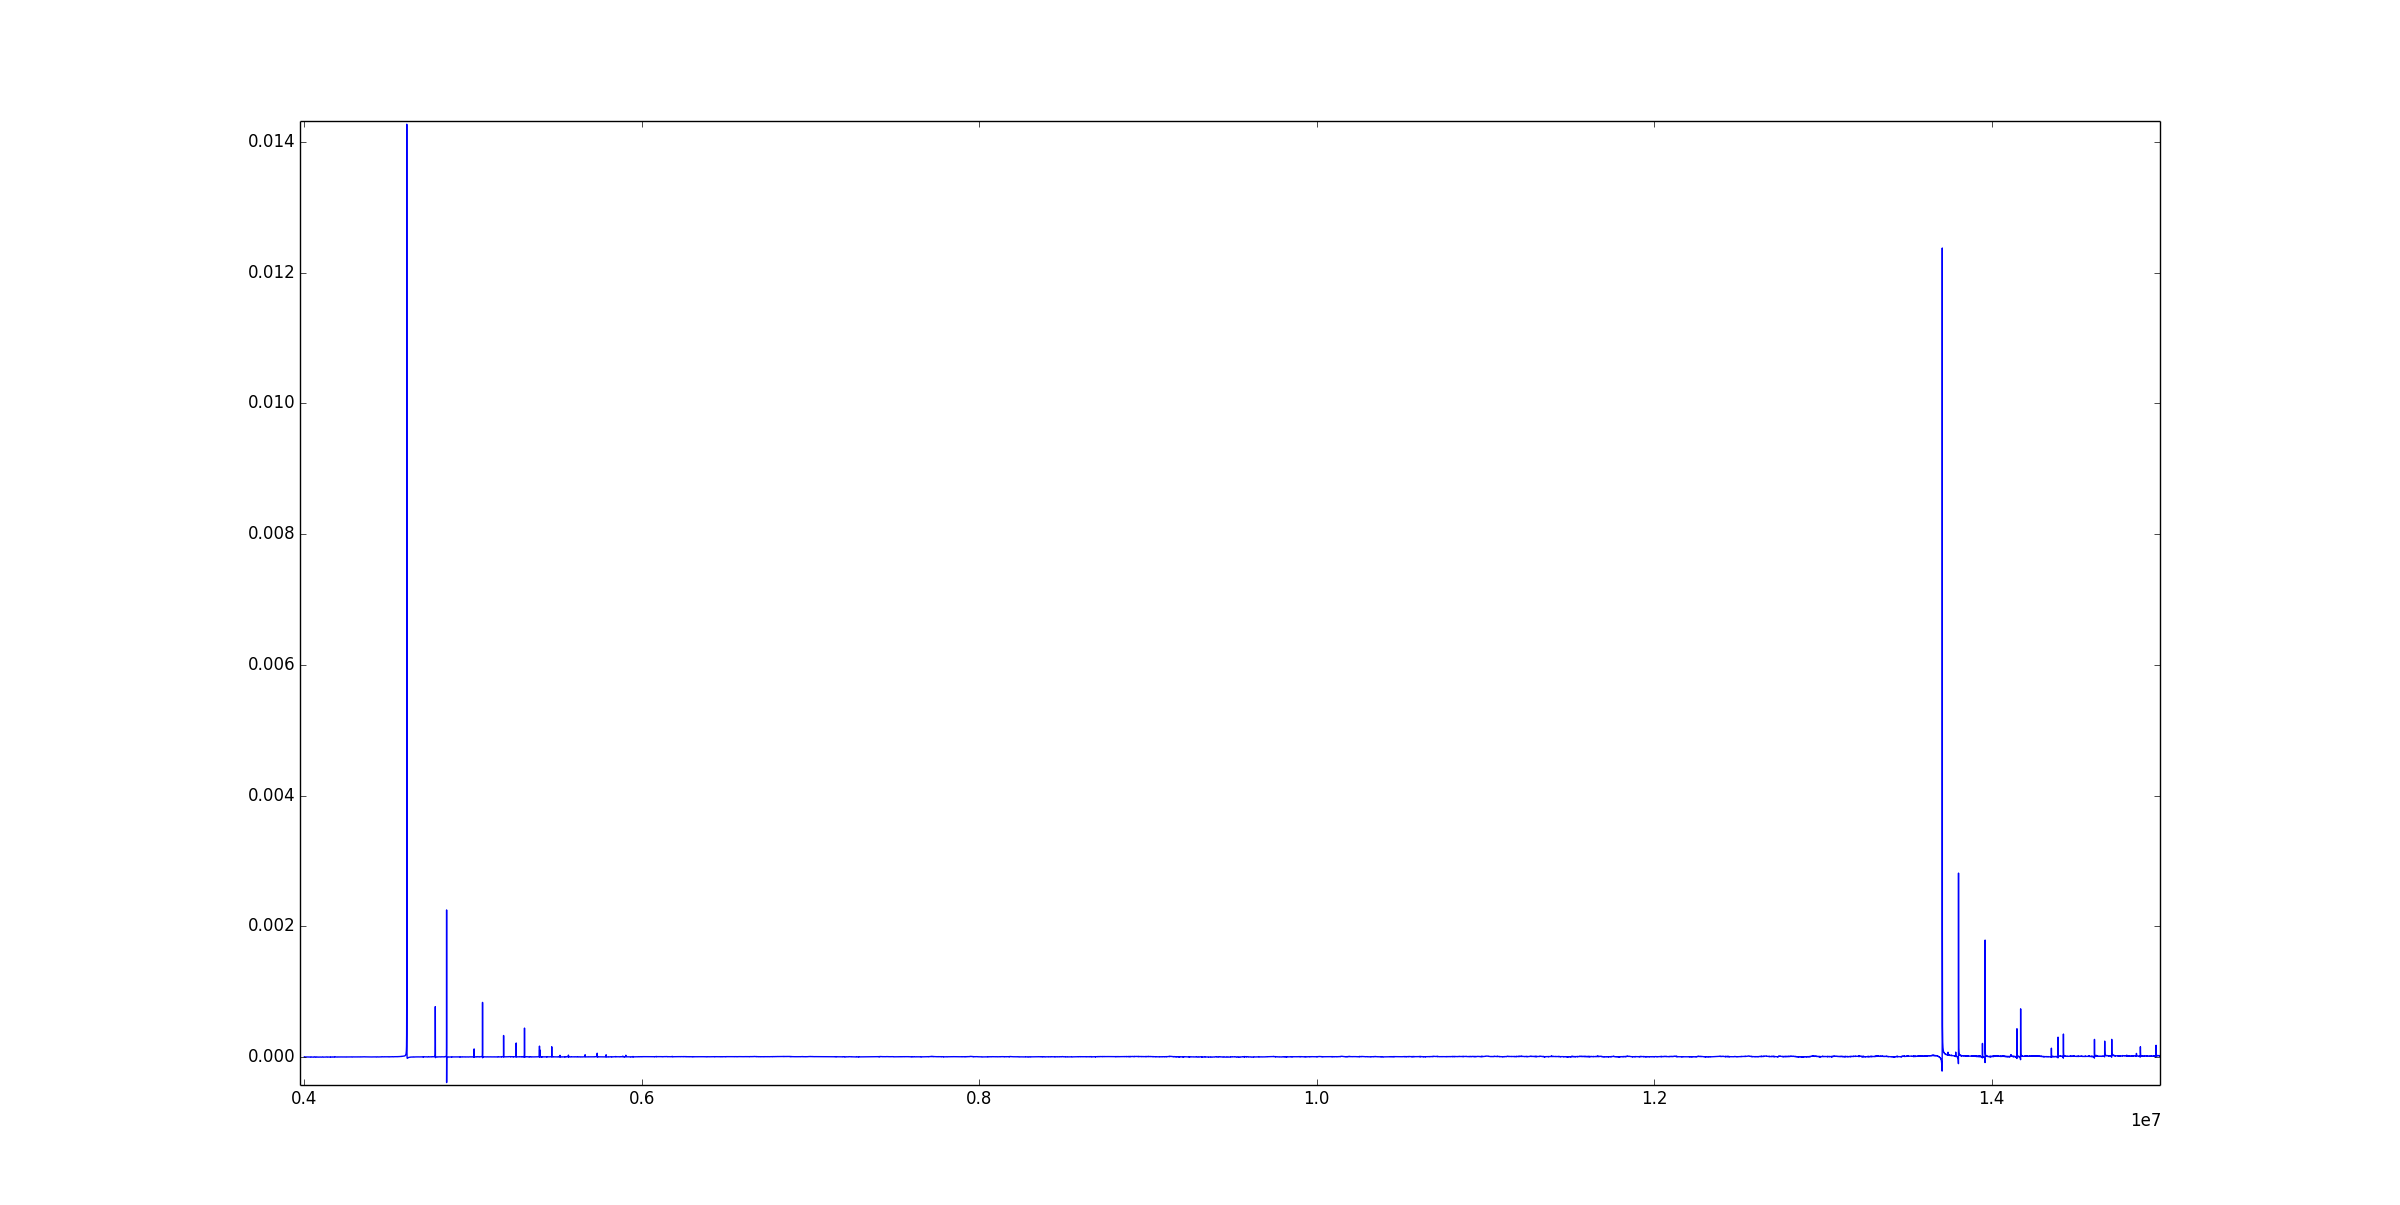
\includegraphics[width=\textwidth]{figures/frequency_scan.png}
	\caption{Frequency scan of the crystal.}
	\label{fig:frequency_scan}
\end{figure}

First of all, a large response means a high current. Apart from the difficulty of making a high frequency source with high current, this leads to several undesirable effects, such as heating up of the crystal [XXX] and high voltage drops in parasitic inductances. When several crystals are paralleled, their currents are summed, which further increases the effect of the parasitic inductance. 

Secondly, the level of aniscochronism seems to be independent of the size of the response. A high level of anisochronism is desirable, since lower amplitudes are needed to reach bistability, which eases the requirements of the driving system. It is also expected that a high level of anisochronism leads to a higher sensitivity to mass. 

Finally, not only do the characteristics of the resonance peak itself (i.e. its size and its level of anisochronism) matter, but also how far it is from its other resonance peaks. Since the crystals will be paralleled, a large area without resonance peaks around the peak that is used for measurement is needed to limit the amount of crosstalk. 

The resonance peak at $f = \SI{4.8}{MHz}$ [XXX] was selected to use for the rest of this experiment. The peak has a high level of anisochronism, while having an amplitude of about 6 times lower than the large main resonance peak at $f_0 = \SI{4.606}{MHz}$. 

\subsection{Amplitude-frequency dependance}

A few frequency responses of an uncoated crystal at different driving powers can be found in \autoref{fig:hysteresis_excerpt}. The crystal shows linear behaviour at low driving amplitudes, but it becomes bistable as the driving amplitude rises. The bistable area in \autoref{fig:hysteresis_regime} is obtained by subtracting the response of the backward sweep from the response of the forward sweep. 

\begin{figure}
	\centering
		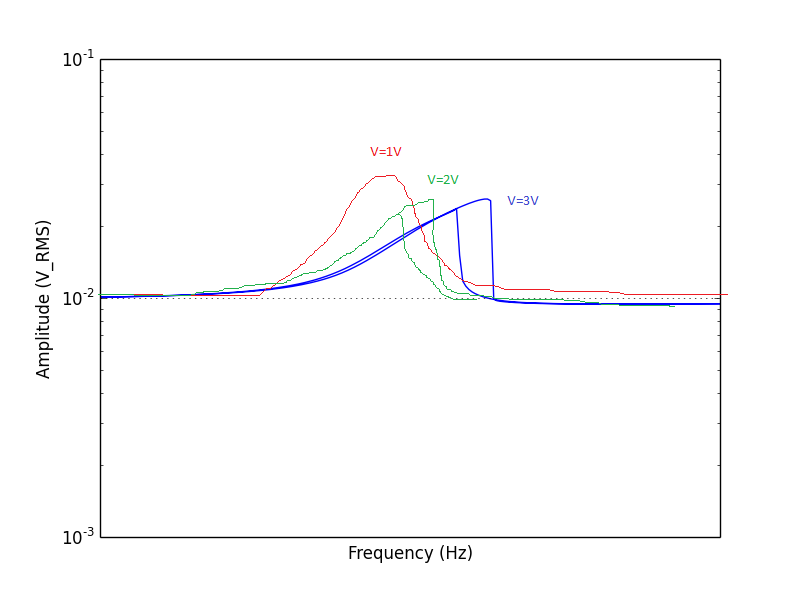
\includegraphics[width=\textwidth]{figures/hysteresis_excerpt.png}
	\caption{Some sweeps at different power XXX}
	\label{fig:hysteresis_excerpt}
\end{figure}

\begin{figure}
	\centering
		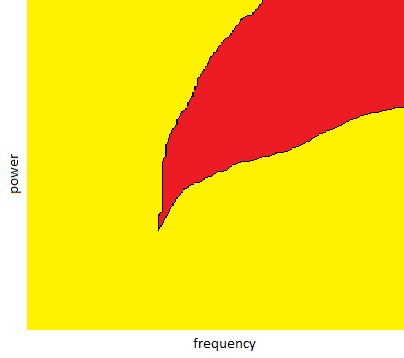
\includegraphics[width=\textwidth]{figures/hysteresis_regime.png}
	\caption{Hysteresis plot of XXX}
	\label{fig:hysteresis_regime}
\end{figure}


In \autoref{fig:hysteresis_excerpt_coatings} some frequency sweeps at different driving powers of four identical crystals with different coatings (PDMS, PEG, PEE and PAA) are displayed alongside their responses before coating. The coating has decreased the resonance frequency of the crystal, as was expected due to mass loading. The Q-factor has also decreased, which can be attributed to losses in the coating. A third observation is that the anisochronic effect has decreased. This can be explained by the lower Q-factor. The amplitude of mechanical movement, and therefore the significance of non-linear effects, is smaller due to the higher damping. The new bistable areas can be found in \autoref{fig:hysteresis_regime_coated}, alongside their old bistable areas in dashes. 

\begin{figure}
	\centering
  \begin{subfigure}[b]{\textwidth}
		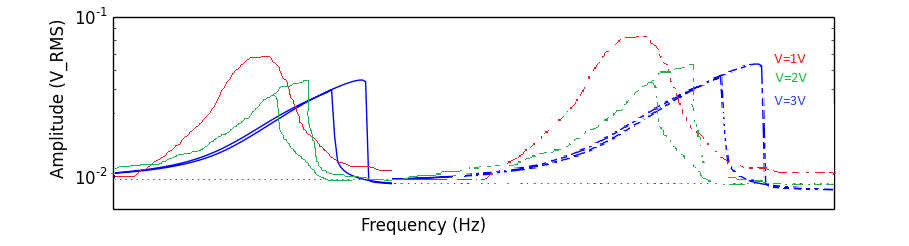
\includegraphics[width=\textwidth]{figures/hysteresis_excerpt_coated.png}
		\caption{PDMA}
		\label{fig:PDMA}
  \end{subfigure}
	
	  \begin{subfigure}[b]{\textwidth}
		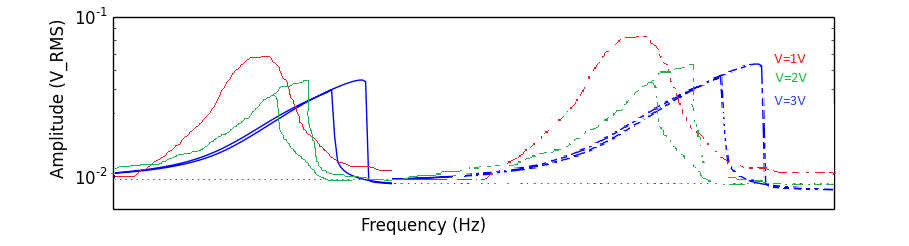
\includegraphics[width=\textwidth]{figures/hysteresis_excerpt_coated.png}
		\caption{PEG}
		\label{fig:PEG}
  \end{subfigure}
		
	  \begin{subfigure}[b]{\textwidth}
		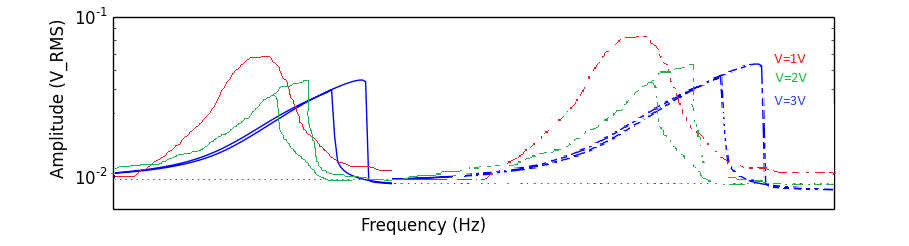
\includegraphics[width=\textwidth]{figures/hysteresis_excerpt_coated.png}
		\caption{PEE}
		\label{fig:PEE}
  \end{subfigure}
		
	  \begin{subfigure}[b]{\textwidth}
		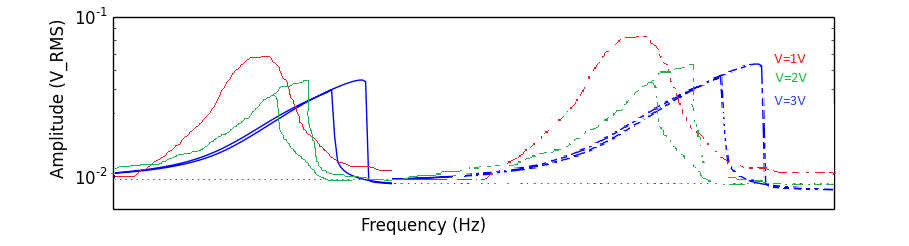
\includegraphics[width=\textwidth]{figures/hysteresis_excerpt_coated.png}
		\caption{PAA}
		\label{fig:PAA}
  \end{subfigure}
	\caption{A few frequency responses of four identical crystals with different coatings alongside their original responses before coating (dashed).}
	\label{fig:hysteresis_excerpt_coatings}
\end{figure}

\begin{figure}
	\centering
  \begin{subfigure}[b]{0.4\textwidth}
		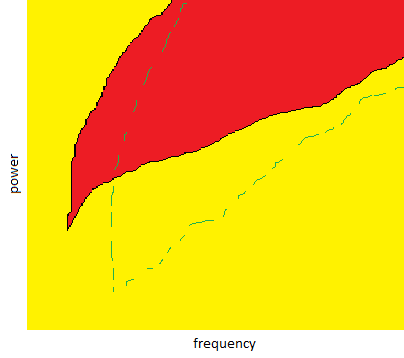
\includegraphics[width=\textwidth]{figures/hysteresis_regime_coated.png}
		\caption{PDMA}
		\label{fig:rPDMA}
  \end{subfigure}
	  \begin{subfigure}[b]{0.4\textwidth}
		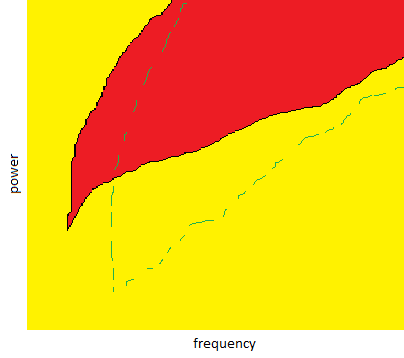
\includegraphics[width=\textwidth]{figures/hysteresis_regime_coated.png}
		\caption{PEG}
		\label{fig:rPEG}
  \end{subfigure}
		
	  \begin{subfigure}[b]{0.4\textwidth}
		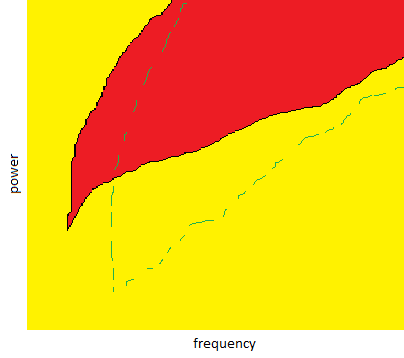
\includegraphics[width=\textwidth]{figures/hysteresis_regime_coated.png}
		\caption{PEE}
		\label{fig:rPEE}
  \end{subfigure}
	  \begin{subfigure}[b]{0.4\textwidth}
		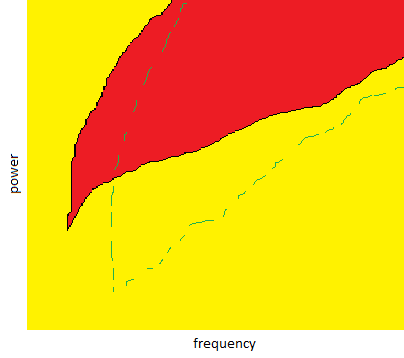
\includegraphics[width=\textwidth]{figures/hysteresis_regime_coated.png}
		\caption{PAA}
		\label{fig:rPAA}
  \end{subfigure}
	
	\caption{Bistable regime before (dashed) and after coating for four identical crystals with different coatings. }
	\label{fig:hysteresis_regime_coated}
\end{figure}

\autoref{fig:parallel} shows the frequency response at a constant driving amplitude of four crystals with closely spaced resonance frequencies placed in parallel, alongside the four individual responses of the crystals. The jump points of the parallel response are to the jump points of the individual crystals, but not quite identical. There are two factors which give rise to this behaviour. Firstly there will always be some crosstalk between the crystals, since the driving circuit is not a perfect voltage source. Secondly, since this experiment is conducted in open air, fluctuations in temperature and humidity are responsible for a different outcome of each measurement. 

As the jump points of the frequency response will shift when a gas is sensed, the crosstalk will manifest itself differently for different mixtures of gasses, so it will always degrade the measurement in an unpredictable way. The error due to fluctuations in temperature and humidity can be minimized by repeating the measurement and averaging the results. 

\begin{figure}
	\centering
		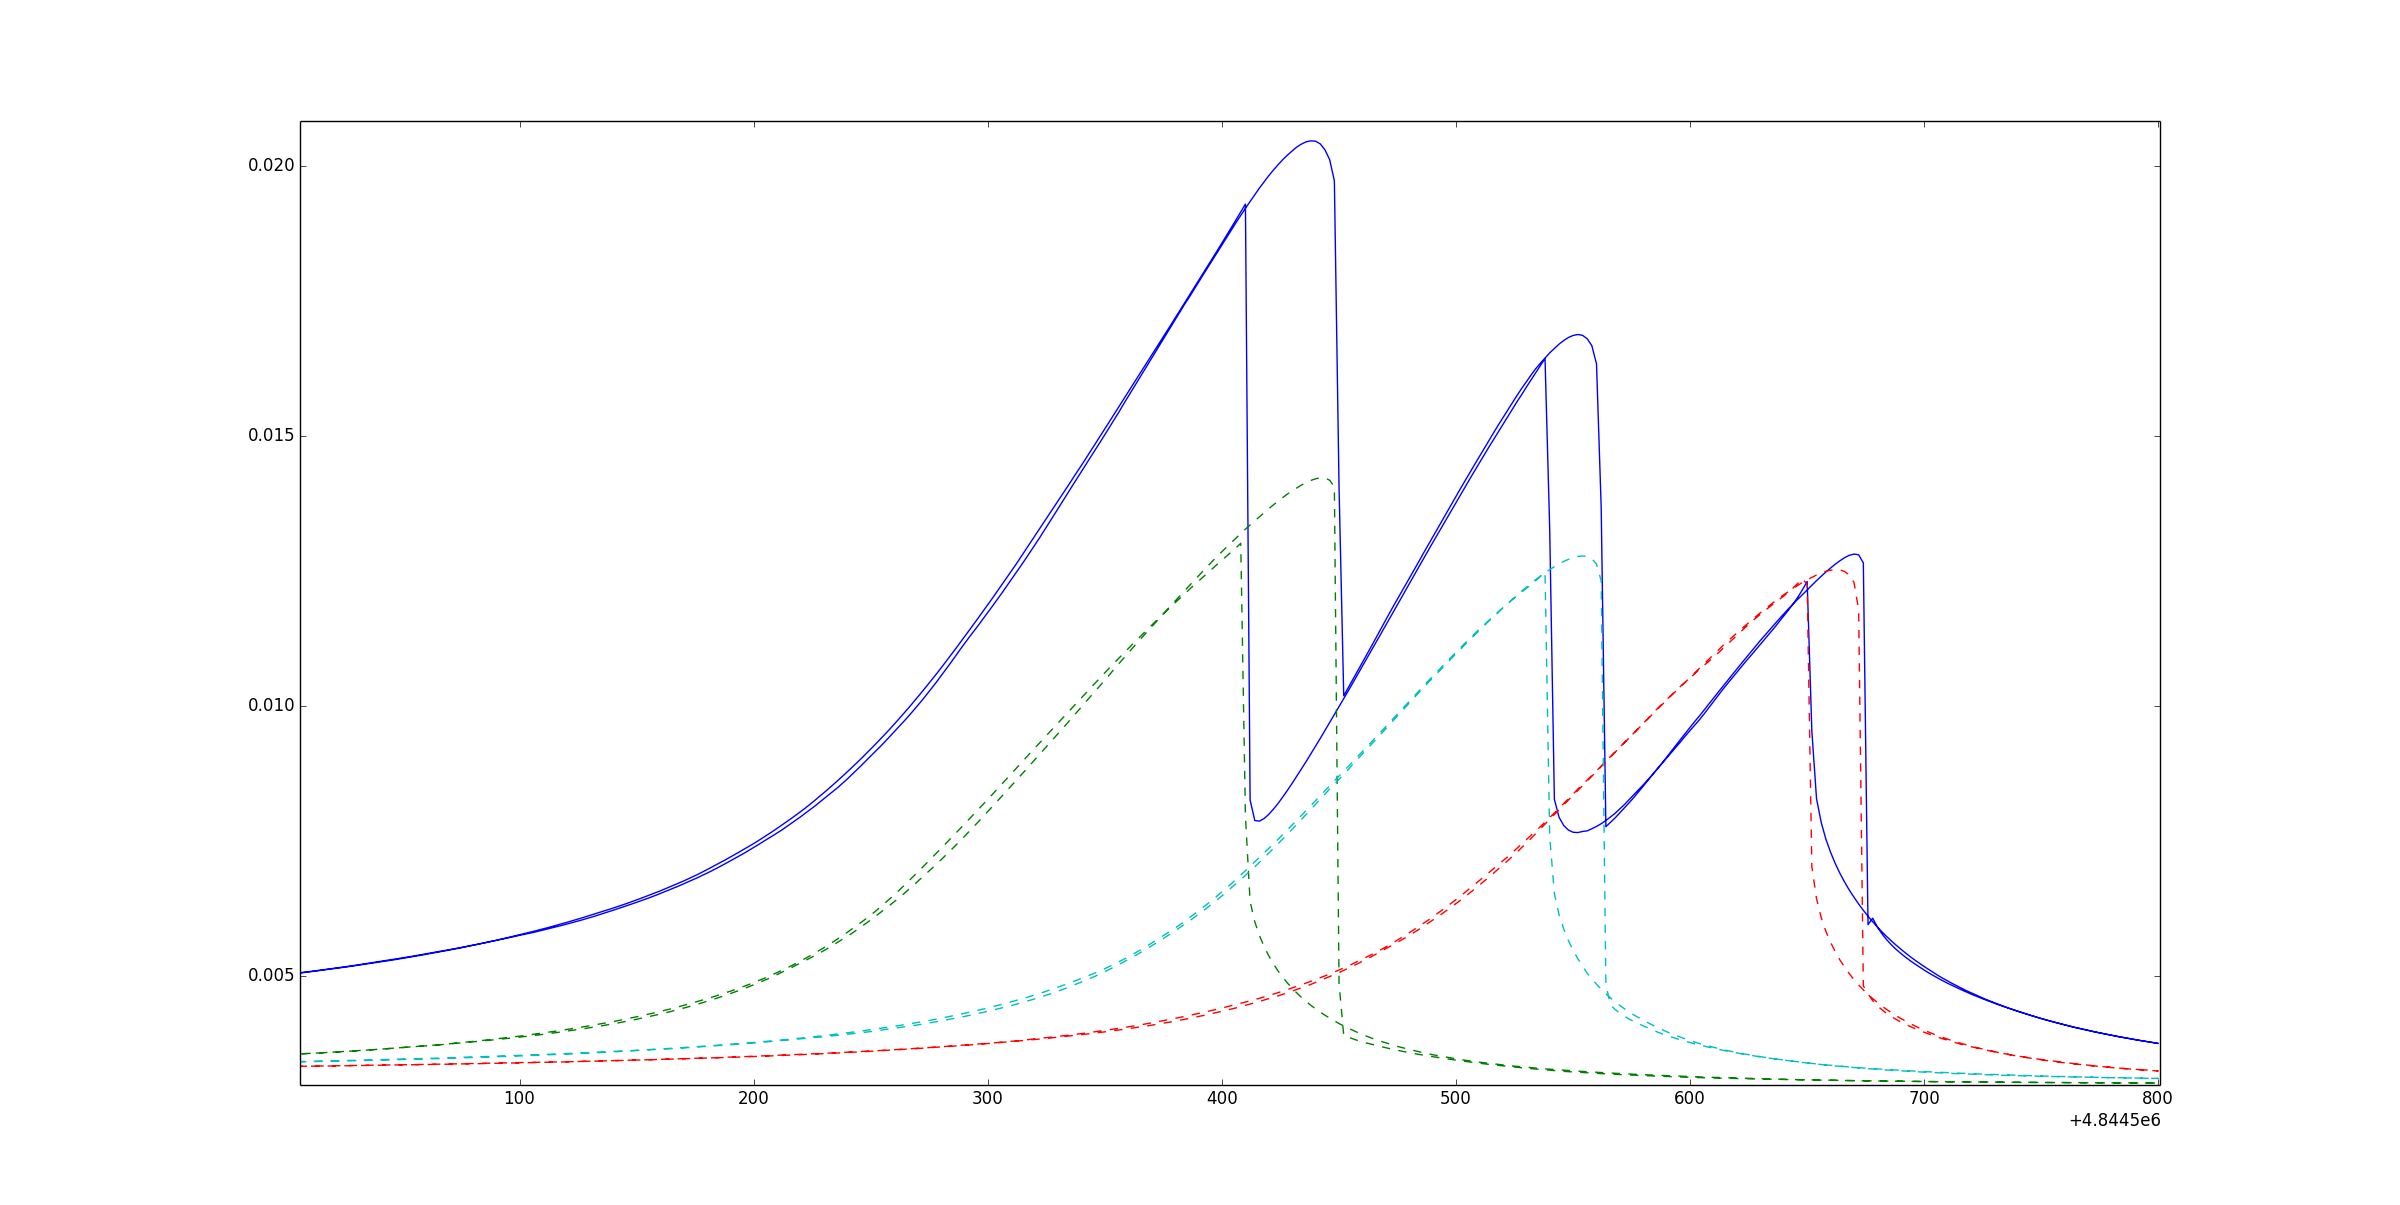
\includegraphics[width=\textwidth]{figures/parallel.png}
	\caption{The frequency response of three parallel uncoated crystals with closely spaced resonance frequencies. The driving amplitude is $V_p = \SI{3.25}{V}$. The frequency responses of the individual crystals are dashed.}
	\label{fig:parallel}
\end{figure}

\subsection{Gas sensing}


